% while : ; do pkill -SIGHUP mupdf ; sleep 7 ; done
%%%%%%%%%%%%%%%%%%%%%%%%%%%%%%%%%%%%%%%%%%%%%%%%%%%%%%%%%%%%%%%%%%%%%%%%%%%%%%%%
% Format du document.
\documentclass[a4paper,12pt]{article}

% Paquets utilisés
\usepackage{float}
\usepackage{lmodern}
\usepackage{fancyhdr}
\usepackage{geometry}
\usepackage{graphicx}
\usepackage{hyperref}
\usepackage{verbatim}
\usepackage{microtype}
\usepackage[T1]{fontenc}
\usepackage[french]{babel}
\usepackage[utf8]{inputenc}

% Paramètres du titre.
\title{\textbf{Network Simulator 2 - Utilisation Basique}}
\author{Abdellah Elazzam}
\date{\small{\textit{Novembre 2017}}}

% Paramètres des hyperliens.
\hypersetup{
 colorlinks = true,
 breaklinks = true,
 urlcolor   = blue,
 linkcolor  = blue,
 citecolor  = green
}

% Paramètres de disposition géométrique.
\geometry{
 left   = 2cm,
 right  = 2cm,
 top    = 2cm,
 bottom = 2cm
}

% https://tex.stackexchange.com/questions/197174/renewcommand-labelitem-doesnt-work-with-multiple-languages
\frenchbsetup{StandardItemLabels=true}

% Pas de numérotation des pages.
\pagestyle{empty}

%%%%%%%%%%%%%%%%%%%%%%%%%%%%%%%%%%%%%%%%%%%%%%%%%%%%%%%%%%%%%%%%%%%%%%%%%%%%%%%%
\begin{document}

\maketitle
\thispagestyle{empty}

\section{Congestions et flux TCP:}
\subsection{Paramètres de simulation:}
\begin{figure}[H]
\centering
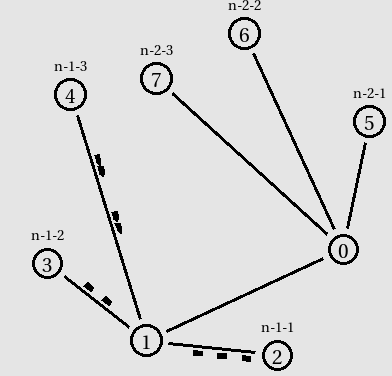
\includegraphics[width=8cm]{img/topologie.png}
\caption{Topologie à huit noeuds avec un lien de coeur BottleNeck}
\end{figure}
\medbreak
\begin{itemize}
\item \texttt{TCP émetteurs:} Node1,Node2,Node3 
\item \texttt{TCP émetteurs:} bandwidth/delay:5Mb,5ms(variable)
\item \texttt{Bottleneck-link:} bandwidth/delay:10Mb,5ms
\item \texttt{TCP récepteurs(Sinks):} Node5,Node6,Node7 
\item \texttt{Queue Management:} Drop-tail
\item \texttt{Queue limits:} 10
\item \texttt{Packet size:} Taille des paquets émis 1500 (MTU)
\item \texttt{Data Sent:} 40000000
\item \texttt{Observation period:} 0-50
\item \texttt{TCP Type:} Tahoe-Reno-Cubic

\end{itemize}

\subsection{TCP Tahoe:}
\subsubsection{Équité:}
\begin{figure}[H]
\centering
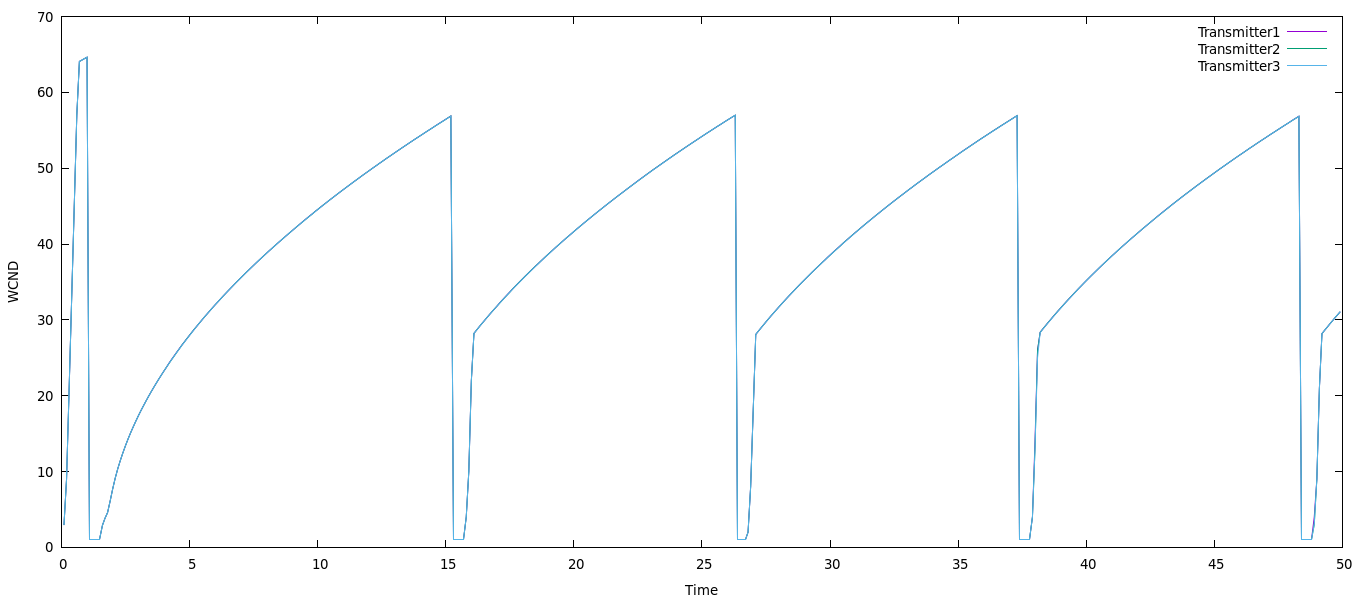
\includegraphics[width=16cm]{img/Tahoe.png}
\caption{Evolution de la fenêtre de congestion pour le TCP Tahoe}
\end{figure}
La variante TCP pour les trois émetteurs est la même. Il s'agit de Tahoe, la version par défault de ns2.On remarque bien que le contrôle de la congestion de TCP converge pour fournir une part égale de la bande passante d'un lien de goulot d'étranglement pour les trois connexions TCP concurrentes. Une fois que la congestion survient le CWND revint à 1 et commence le Slow Start. En fait la congestion apparaît car le débit utile du flux d’entrée (ici correspond à la somme des troix débit des flux d'entrées ) est supérieure au débit utile de sortie qui est celle du lien de cœur.
\subsubsection{Débit Utile:}
Le débit utile (ou throughput) est le débit total en réception. Il est calculé pour un  intervalle 
de temps, en divisant la quantité totale d’information reçue pendant cet  intervalle, par la durée de 
l’intervalle en question. La formule générale pour le calcul du débit utile est ainsi :  
\begin{center}
$throughput=\frac{nombre \ des \ Bytes \ recus \ pendant\ \delta t }{\delta t}$
\end{center}
\begin{figure}[H]
\centering
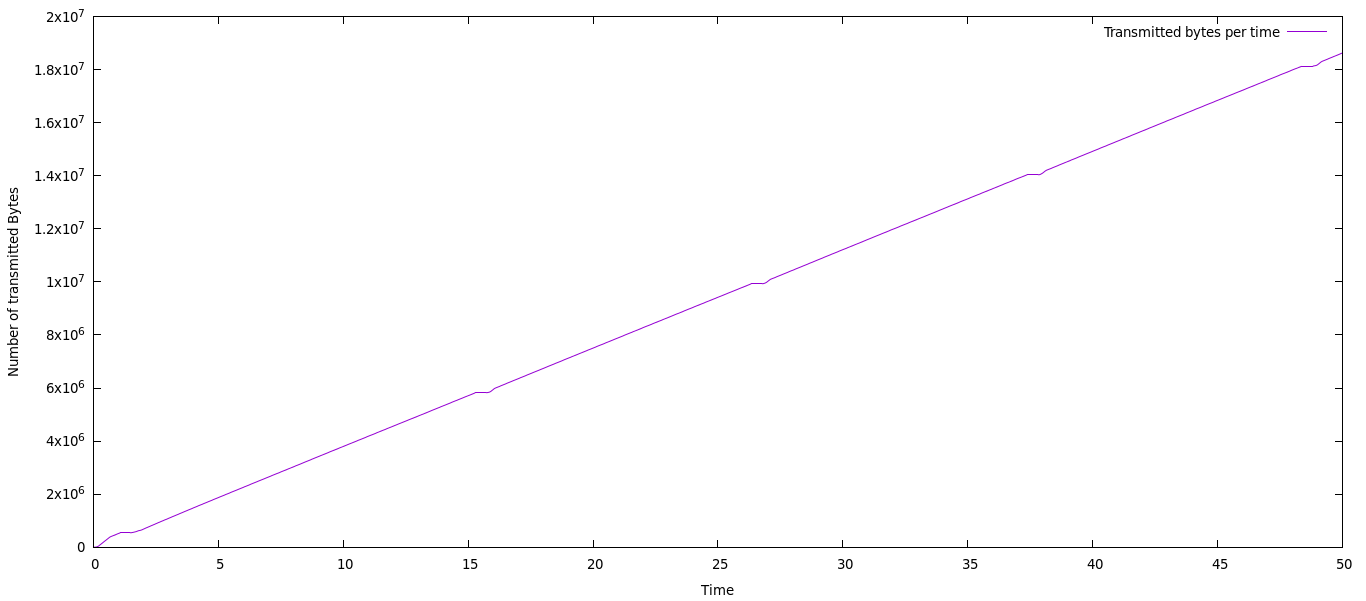
\includegraphics[width=16cm]{img/paquets_received_tahoe.png}
\caption{Nombre de paquets en transit dans le lien de cœur au cours du temps}
\end{figure}
Le débit théorique du lien de goulot d'étranglement est de \texttt{10 Mbps} calculé a partir de la configuration de notre réseau.\\
Le débit utile du lien de goulot d'étranglement est de : 
\begin{center}
	$\frac{18628600*8}{50} = 2.98 Mbps$ 
\end{center}
Le TCP Tahoe permet de transmettre les données avec un facteur proche d'un quart par rapport au débit théorique.  .


\subsection{TCP Reno:}
\subsubsection{Équité:}
On reprend avec la variante TCP Reno. On implémente l'agent TCP Reno sur le premier lien émetteur en gardant les deux autres émetteurs sur Tahoe.
\begin{figure}[H]
\centering
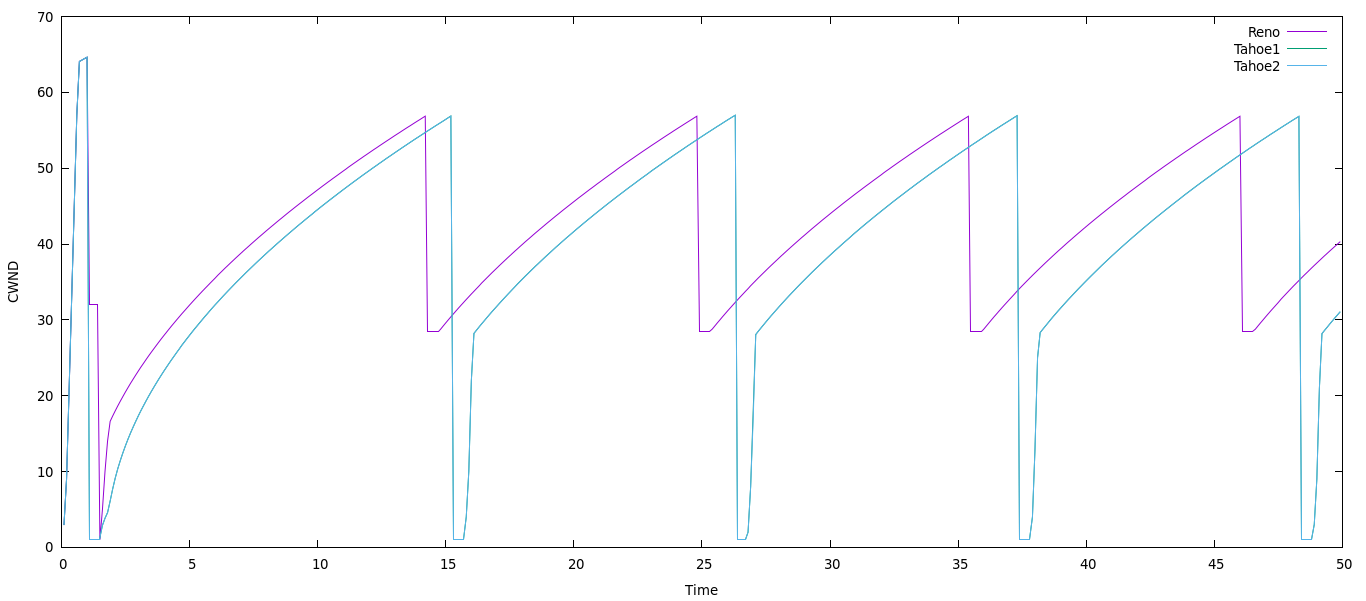
\includegraphics[width=16cm]{img/tahoevsreno.png}
\caption{L'évolution de la fenêtre de congestion au cours du temps selon  deux variantes TCP Reno/Tahoe}
\end{figure}
On remarque que la congestion pour Reno est différente à celle de Tahoe. Reno permet de ne pas repartir en Slow Start (et avec un cwnd à 1) dès qu'il y a congestion mais plutôt diminuer de moitié la valeur de cwnd. Les débits sont donc plus stables. Par contre, le défaut de ces deux algorithmes c'est qu'ils remplissent le Bottle-Neck complètement avant de réagir.
\subsubsection{RTT:}
Tous les émetteurs sur l'algorithme Reno. On change le RTT pour des valeurs : \texttt{5ms,10ms,20ms}.
\begin{figure}[H]
\centering
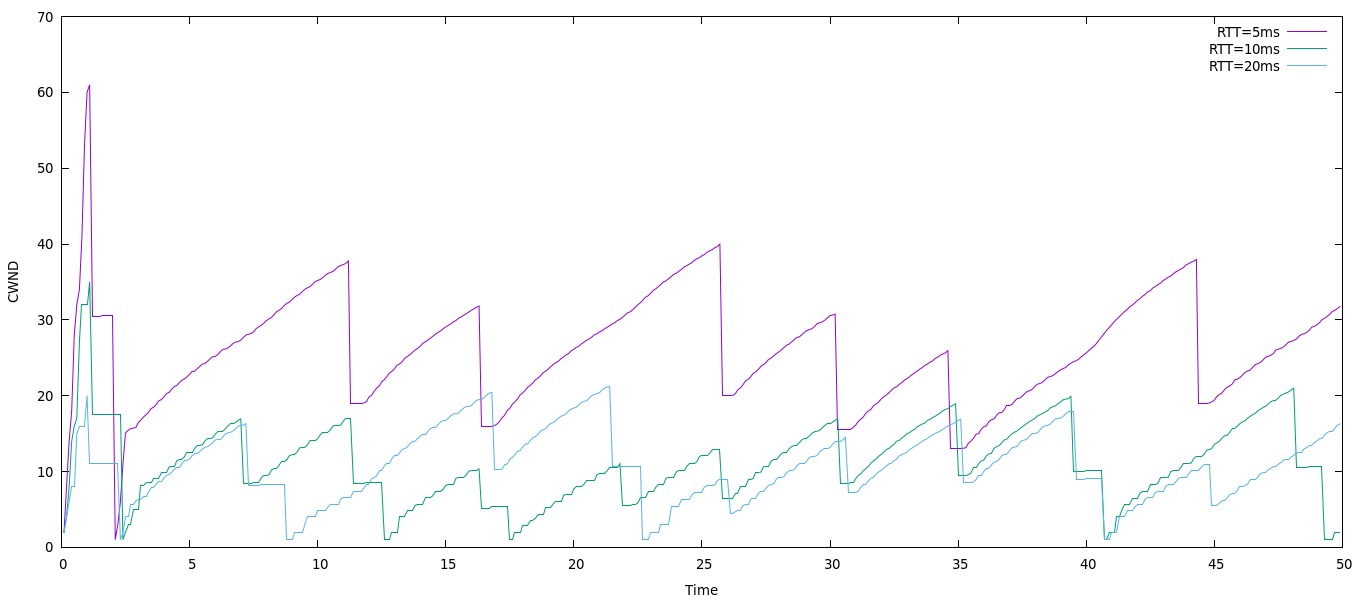
\includegraphics[width=16cm]{img/RTT_Reno.png}
\caption{L'évolution de la fenêtre de congestion au cours du temps selon plusieurs RTT}
\end{figure}
On remarque que l'algorithme Reno n'est pas optimal pour de grands RTT. Ainsi, il est pas adapté aux réseaux High bandwidth et High RTT.
\subsubsection{Débit Utile:}
La version TCP est la même pour les trois émetteurs a savoir Reno. On voit que la courbe suivante ne change pas beaucoup par rapport à celle de Tahoe, ainsi j'ai opté a la création d'un moniteur permettant d'avoir le nombre exacte de bytes reçus dans le lien de cœur à la fin de simulation (ici \texttt{18628600 Bytes}).  
\begin{figure}[H]
\centering
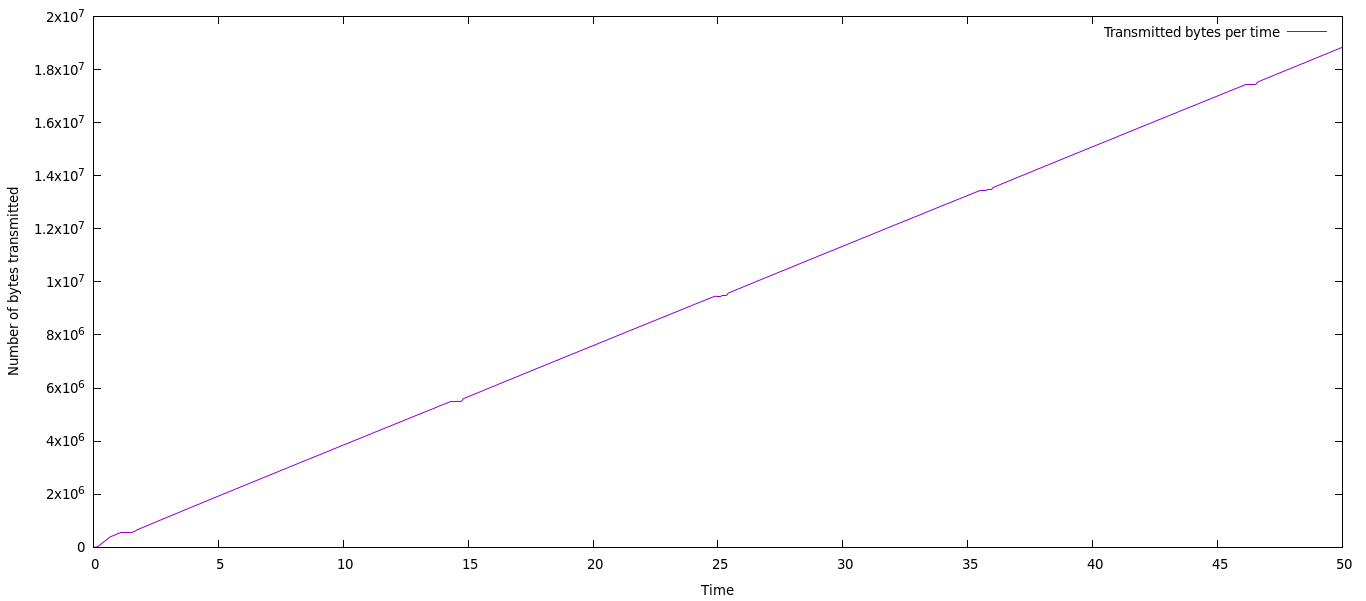
\includegraphics[width=16cm]{img/paquets_received_reno.png}
\caption{Nombre de paquets en transit dans le lien de cœur au cours du temps}
\end{figure}
Le débit utile du lien de goulot d'étranglement est de : 
\begin{center}
	$\frac{18628600*8}{50} = 3.01 Mbps$ 
\end{center}
Le TCP Reno permet d'optimiser le débit utile par rapport à la version Tahoe grâce à sa phase de Fast Recovery qui permet d'augmenter l'aire sous la courbe de la fenêtre de congestion .

\subsection{TCP Cubic:}
\subsubsection{Équité:}
On implémente l'agent TCP Cubic sur le premier transmetteur, Reno sur le deuxième transmiteur, et Tahoe sur le troixième.
\begin{figure}[H]
\centering
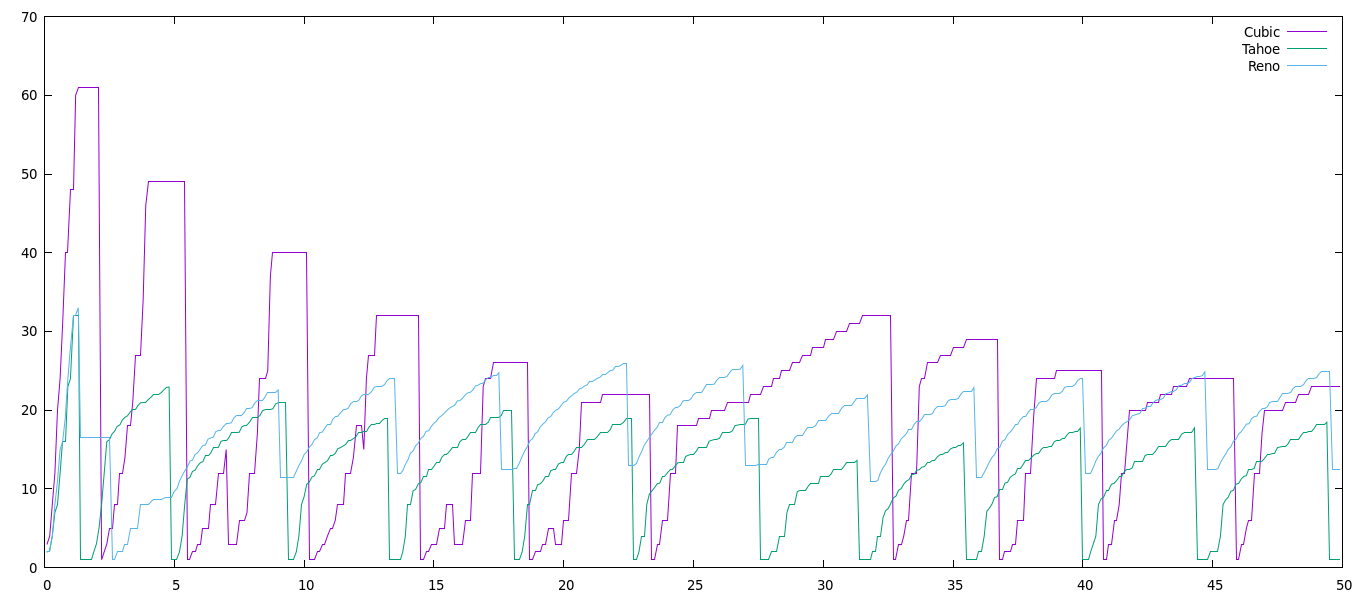
\includegraphics[width=16cm]{img/cubic_reno_tahoe.png}
\caption{L'évolution de la fenêtre de congestion au cours du temps selon trois variantes TCP Reno/Tahoe}
\end{figure}
Cubic permet une bonne équité, il est stable en maintenant un haut débit et qu'il permet une bonne mise à l'échelle.L'algorithme fait attention à ne pas trop augmenter cwnd, aussi si lors de notre recherche on fait des sauts trop grands (défini par un certain seuil), on préfèrera accroître cwnd de manière logarithmique. Cubic a une phase montante douce, ce qui le rend plus « amical » envers les autres versions de TCP.
\subsubsection{RTT:}
Tous les émetteurs sur l'algorithme Cubic. On change le RTT pour des valeurs : \texttt{30ms,40ms,50ms}.
\begin{figure}[H]
\centering
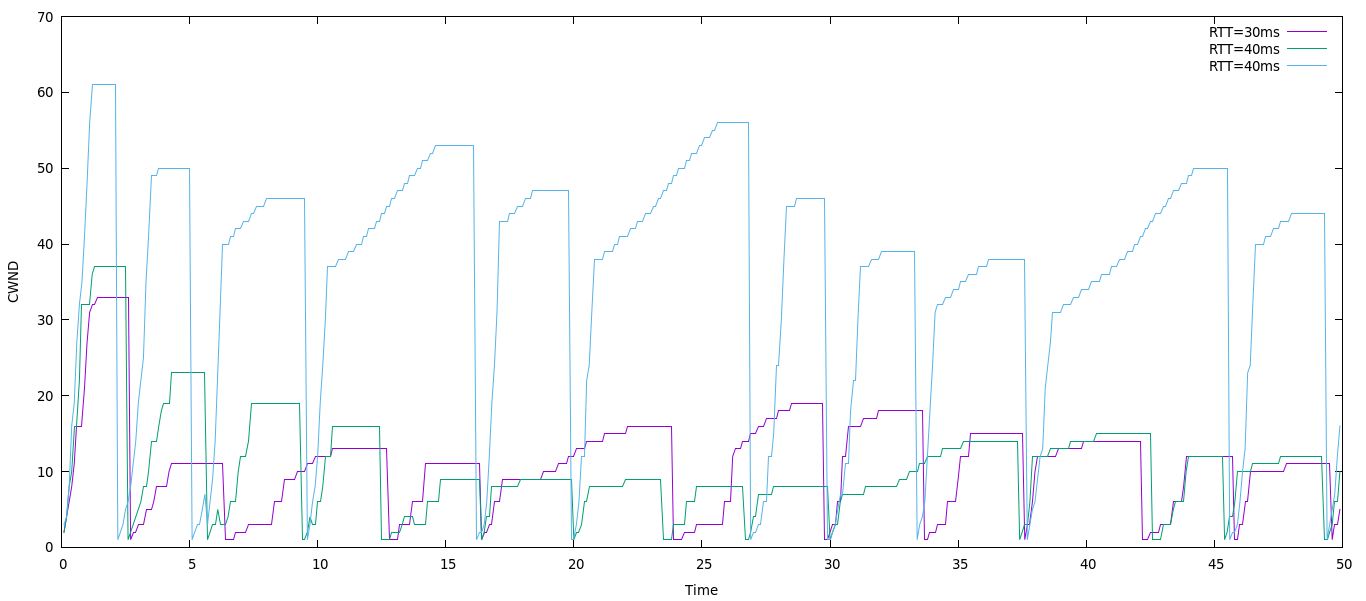
\includegraphics[width=16cm]{img/RTT_Cubic.png}
\caption{L'évolution de la fenêtre de congestion au cours du temps selon plusieurs RTT}
\end{figure}
	La fonction de croissance de CUBIC augmente la fenêtre de congestion en fonction du temps écoulé
de la dernière époque de congestion. Ainsi, le protocole peut être très équitable au niveau du RTT (RTT-Fairness) vue que le taux de croissance de la fenêtre est déterminé plus par le temps écoulé. Comme c'est moins dépendante de RTT, le protocole peut se permettre d'être plus évolutif sans décroître l'équité du RTT. En outre, cette fonctionnalité permet plus de convivialité TCP: le protocole est conçu ainnsi pour bien évoluer dans les réseaux RTT long, tout en restant amical pour les autres algorithmes pour des Short-RTT où la fonction de croissance cubique est beaucoup plus lente.
\subsubsection{Débit Utile:}
La version TCP est la même pour les trois émetteurs a savoir Cubic. On voit que la courbe suivante ne change pas beaucoup par rapport à celle de Tahoe,le moniteur permet d'avoir le nombre exacte de bytes reçus dans le lien de cœur à la fin de simulation (ici \texttt{22175320 Bytes}).  
\begin{figure}[H]
\centering
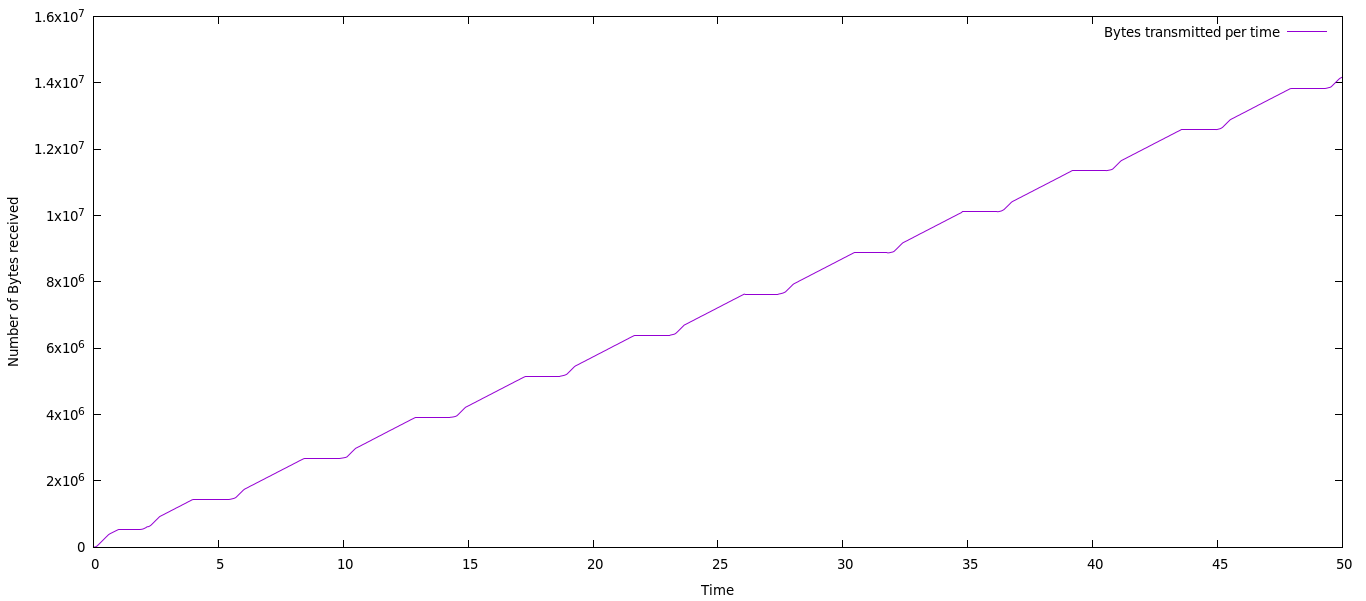
\includegraphics[width=16cm]{img/paquets_received_cubic.png}
\caption{Nombre de paquets en transit dans le lien de cœur au cours du temps pour la version Cubic}
\end{figure}
Le débit utile du lien de goulot d'étranglement est de : 
\begin{center}
	$\frac{22175320*8}{50} = 3.54 Mbps$ 
\end{center}
On voit bien que le débit utile est optimisé par rapport aux autres algorithmes précédentes. Ceci se voit clairement dans la figure où l'aire sous la courbe est grand.


\end{document}
%%%%%%%%%%%%%%%%%%%%%%%%%%%%%%%%%%%%%%%%%%%%%%%%%%%%%%%%%%%%%%%%%%%%%%%%%%%%%%%%
